\documentclass{beamer}
\usepackage[utf8]{inputenc}
\usepackage{graphicx}
\usepackage{xspace} % Needed for macro \xspace

% Remove navigation controls
\usenavigationsymbolstemplate{}

% Slide numbering
\setbeamertemplate{footline}[frame number]

% Convienence macro
\newcommand{\atweb}{\textbf{@Web}\xspace}

% Macro for writing an RDF triplet
\newcommand{\triplet}[1]{$\langle$\texttt{#1}$\rangle$}

\title{An introduction to the semantic web technologies}
\subtitle{And their use within the \atweb platform}
\author{
  Leandro Lovisolo \\
  \footnotesize{\href{mailto:leandro.lovisolo@supagro.inra.fr}
                     {leandro.lovisolo@supagro.inra.fr}}
}
\date{September 23, 2015}
\institute{
  INRA SupAgro and INRIA GraphiK \\
  Montpellier, France
}

\begin{document}

\begin{frame}
  \titlepage
\end{frame}

\begin{frame}
  \frametitle{Outline of the presentation}

  \begin{itemize}
    \item What's an ontology?
    \item RDF
    \item RDFS
    \item OWL
    \item SKOS
    \item SPARQL
    \item The n-ary relationship pattern used in \atweb
    \item Examples of tables in scientific documents annotated using n-ary
      relationships in \atweb
  \end{itemize}
\end{frame}

\begin{frame}
  \frametitle{What's an ontology?}

  \pause

  It's a formal description of a domain of interest based on:

  \pause

  \begin{itemize}
    \item a set of \textit{individuals} (also called entities or objects),

    \pause

    \item a set of \textit{classes} of individuals, and

    \pause

    \item a set of \textit{relationships} (sometimes called properties)
      between these individuals;
  \end{itemize}

  \pause

  and a set of logical constraints to specify, among other things:

  \pause

  \begin{itemize}
    \item class membership,

    \pause

    \item subclass/subproperty relationships,

    \pause

    \item domain/range restrictions on properties,

    \pause

    \item cardinality constraints,

    \pause

    \item class union/intersection/disjointness constraints,

    \pause

    \item etc.
  \end{itemize}
\end{frame}

\begin{frame}
  \frametitle{Web resources, URI, namespaces}

  A \textit{resource} is anything that can be referred to: a web page, a
  person, a city, a university course, etc.

  \pause

  \medskip

  Resources are identified by \textit{URIs}, for example:

  \begin{itemize}
    \item \texttt{http://example.com/MyOntology},
    \item \texttt{http://example.com/MyOntology\#Leandro},
    \item \texttt{http://example.com/MyOntology\#Pizza},
    \item etc.
  \end{itemize}

  \pause

  To avoid carrying long URIs, \textit{namespaces} are used. \pause Thus,

  \pause

  \begin{itemize}
    \item \texttt{http://example.com/MyOntology} \pause \hfill becomes

    \pause

    \item \texttt{example:MyOntology} \pause \hfill abbreviated as

    \pause

    \item \texttt{:MyOntology}
  \end{itemize}

  \pause

  if \texttt{example} is the default namespace.
\end{frame}

\begin{frame}
  \frametitle{RDF}

  A simple language for describing \textit{annotations} about Web resources
  identified by URIs, from now on referred to as \textbf{facts}.
\end{frame}

\begin{frame}
  \frametitle{RDF}
  \framesubtitle{Triplets}

  Facts are stated as \textit{RDF triplets}.

  \pause

  \medskip

  A triplet is made of a \textit{subject}, a \textit{predicate} and an
  \textit{object}.

  \pause

  \medskip

  Some examples:

  \pause

  \begin{itemize}
    \item \triplet{:Dupond :Leads :InfoDept}

    \pause

    \item \triplet{:Dupond :TeachesIn :UE111}

    \pause

    \item \triplet{:Dupond :TeachesTo :Pierre}

    \pause

    \item \triplet{:Pierre :EnrolledIn :InfoDept}

    \pause

    \item \triplet{:Pierre :RegisteredTo :UE111}

    \pause

    \item \triplet{:UE111 :OfferedBy :InfoDept}
  \end{itemize}
\end{frame}

\begin{frame}
  \frametitle{RDF}
  \framesubtitle{Graph representation}

  \begin{center}
    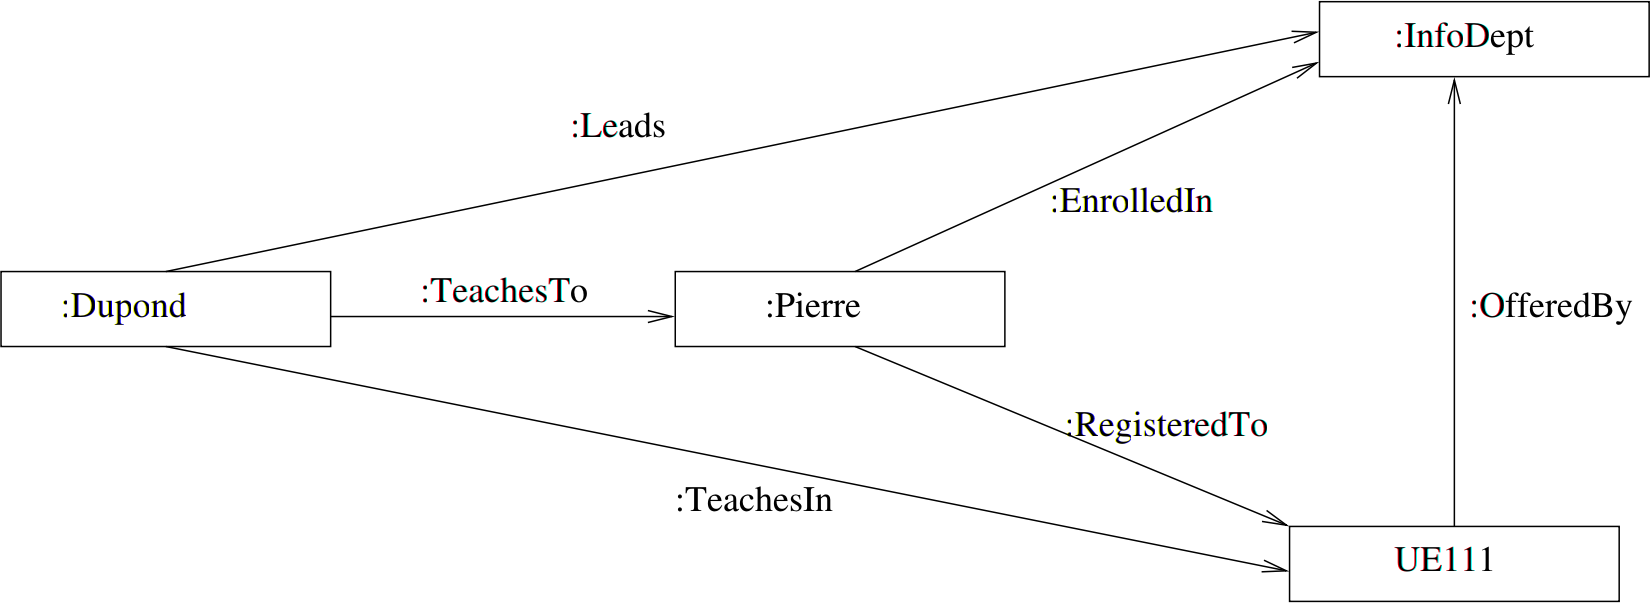
\includegraphics[width=11cm]{graph.png}
  \end{center}

  \triplet{:Dupond :Leads :InfoDept} \\
  \triplet{:Dupond :TeachesIn :UE111} \\
  \triplet{:Dupond :TeachesTo :Pierre} \\
  \triplet{:Pierre :EnrolledIn :InfoDept} \\
  \triplet{:Pierre :RegisteredTo :UE111} \\
  \triplet{:UE110 :OfferedBy :InfoDept}
\end{frame}

\begin{frame}
  \frametitle{RDF}
  \framesubtitle{Syntax}

  There are many different syntaxes for writing RDF triplets, including:

  \pause

  \begin{itemize}
    \item XML (as used in \atweb),

    \pause

    \item Turtle,
    \item N-Triples,
    \item N-Quads,
    \item etc.
  \end{itemize}

  \pause

  However, we're going to focus on the abstract \triplet{subject, predicate,
  object} syntax during this presentation.
\end{frame}

\begin{frame}
  \frametitle{RDFS}

  The \textit{schema language} for RDF. Allows specifying constraints on
  individuals and relationships used in RDF.

  \pause

  \medskip

  Such constraints are:

  \pause

  \begin{itemize}
    \item \texttt{rdf:type} (used to specify class membership of an individual),
    \item \texttt{rdfs:subClassOf} (subclass relationship between classes),
    \item \texttt{rdfs:subPropertyOf} (subproperty relationship between
      properties),
    \item \texttt{rdfs:domain} (domain of a property) and
    \item \texttt{rdfs:range} (range of a property).
  \end{itemize}
\end{frame}

\begin{frame}
  \frametitle{RDFS}
  \framesubtitle{\texttt{rdf:type}}

  Used to specify class membership.

  \pause

  \bigskip

  Syntax: \triplet{i rdf:type C}.

  \pause

  \medskip

  First-order logic translation: $C(i)$.

  \pause

  \bigskip

  Examples:

  \begin{itemize}
    \item \triplet{:Dupond rdf:type :AcademicStaff}
    \item \triplet{:Pierre rdf:type :MasterStudent}
  \end{itemize}
\end{frame}

\begin{frame}
  \frametitle{RDFS}
  \framesubtitle{\texttt{rdfs:subClassOf}}

  Used to specify subclass relationships between classes.

  \pause

  \bigskip

  Syntax: \triplet{C rdfs:subClassOf D}.

  \pause

  \medskip

  First-order logic translation: $\forall X (C(X) \implies D(X))$.

  \pause

  \bigskip

  Example:

  \begin{itemize}
    \item \triplet{:MasterStudent rdfs:subClassOf :Student}
  \end{itemize}

  \pause

  Usage example:

  \begin{itemize}
    \item \triplet{:Pierre rdf:type :MasterStudent}
  \end{itemize}

  \pause

  Which implies:

  \begin{itemize}
    \item \triplet{:Pierre rdf:type :Student}
  \end{itemize}
\end{frame}

\begin{frame}
  \frametitle{RDFS}
  \framesubtitle{\texttt{rdfs:subPropertyOf}}

  Used to specify subproperty relationships between properties.

  \pause

  \bigskip

  Syntax: \triplet{P rdfs:subPropertyOf R}.

  \pause

  \medskip

  First-order logic translation: $\forall X \forall Y (P(X, Y) \implies
                                                       R(X, Y))$.

  \pause

  \bigskip

  Example:

  \begin{itemize}
    \item \triplet{:LateRegisteredTo rdfs:subPropertyOf :RegisteredTo}
  \end{itemize}

  \pause

  Usage example:

  \begin{itemize}
    \item \triplet{:Alice :LateRegisteredTo :UE111}
  \end{itemize}

  \pause

  Which implies:

  \begin{itemize}
    \item \triplet{:Alice :RegisteredTo :UE111}
  \end{itemize}
\end{frame}

\begin{frame}
  \frametitle{RDFS}
  \framesubtitle{\texttt{rdfs:domain}}

  Used to specify the domain of a property.

  \pause

  \bigskip

  Syntax: \triplet{P rdfs:domain C}.

  \pause

  \medskip

  First-order logic translation: $\forall X \forall Y (P(X, Y) \implies C(X))$.

  \pause

  \bigskip

  Example:

  \begin{itemize}
    \item \triplet{:TeachesTo rdfs:domain :AcademicStaff}
  \end{itemize}

  \pause

  Usage example:

  \begin{itemize}
    \item \triplet{:Dupond :TeachesTo :Pierre}
  \end{itemize}

  \pause

  Which implies:

  \begin{itemize}
    \item \triplet{:Dupond rdf:type :AcademicStaff}
  \end{itemize}
\end{frame}

\begin{frame}
  \frametitle{RDFS}
  \framesubtitle{\texttt{rdfs:range}}

  Used to specify the range of a property.

  \pause

  \bigskip

  Syntax: \triplet{P rdfs:range D}.

  \pause

  \medskip

  First-order logic translation: $\forall X \forall Y (P(X, Y) \implies D(Y))$.

  \pause

  \bigskip

  Example:

  \begin{itemize}
    \item \triplet{:TeachesTo rdfs:range :Student}
  \end{itemize}

  \pause

  Usage example:

  \begin{itemize}
    \item \triplet{:Dupond :TeachesTo :Pierre}
  \end{itemize}

  \pause

  Which implies:

  \begin{itemize}
    \item \triplet{:Pierre rdf:type :Student}
  \end{itemize}
\end{frame}

\begin{frame}

\end{frame}

\begin{frame}

\end{frame}

\begin{frame}

\end{frame}

\begin{frame}

\end{frame}

\begin{frame}

\end{frame}

\begin{frame}

\end{frame}

\begin{frame}

\end{frame}

\begin{frame}

\end{frame}

\begin{frame}
  \begin{center}
    \Huge{Thanks!}
  \end{center}
\end{frame}

\end{document}
